\section{Unified Modellig Language}
Til at dokumentere den objektorienteret programmering og udvikling af systemet i denne rapport, anvendes standarden Unified Modelling Language (UML). Ud fra denne standard anvendes modeller til at visualisere struktur og egenskaber af systemet. Måden hvorpå modellerne anvendes, relatere disse sig enten som redskaber til analyse og/eller design af systemet. 
UML modeller inkluderet i denne rapport er:  Use-case (egenskab), Aktivitets- (egenskab) og klasse-diagrammer (struktur).


\subsection{Use-case diagrammer} 
Use-case diagrammer benyttes til at illustrere aktørernes interaktion med et 'system', samt hvordan forskellige use-cases interagere mellem hinanden. Dertil er use-case diagrammet med til at repræsentere funktionelle krav for systemet. Et simpelt eksempel ses af \autoref{fig:use_case} 

\begin{figure} [H]
\centering
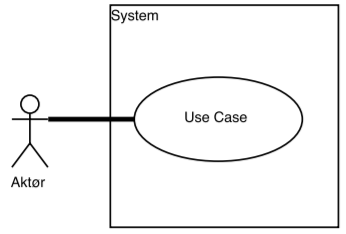
\includegraphics[width=0.5\textwidth]{figures/USE_CASE2}
\caption{Simpelt use-case diagram.}
\label{fig:use_case}
\end{figure}

Af \autoref{fig:xx2} ses aktørens interaktion med use-case visualiseret som en streg mellem de to. I et use-case diagram vil aktøren definere en person/rolle, objekt, eller anden given genstand der kan tilgå system funktionaliteter. Hertil vil den enkelte use-case beskrive en handling eller funktionalitet i systemet. \cite{Fowler2004}


\subsection{Aktivitetsdiagrammer}
Til at beskrive komplekse use-cases eller klassemetoder anvendes aktivitetsdiagrammer. Dette giver overblik over flowet gennem de forskellige aktiviteter i den givne funktion eller metode. \cite{Fowler2004}    

Såfremt der i et aktivitetsdiagram anvendes et 'brille' symbol, indikerer dette at den aktivitet i sig selv er kompleks og er beskrevet i et særskilt aktivitetsdiagram.  

\subsection{Klassediagrammer}
Klassediagrammet vil blive anvendt som et redskab til at designe og give overblik over de forskellige klasser. Hertil vil relationerne mellem de forskellige klasser blive tydeliggjort ved anvendelse af tilhørende symbolisering: nedarvning, association, aggregation, composition mm. Som det ses af \autoref{fig:klassediagram} beskrives hver klasse ud fra et unik klassenavn hvor der yderligere kan tildeles attributter og metoder til den givne klasse. \cite{Fowler2004} 

\begin{figure} [H]
\centering
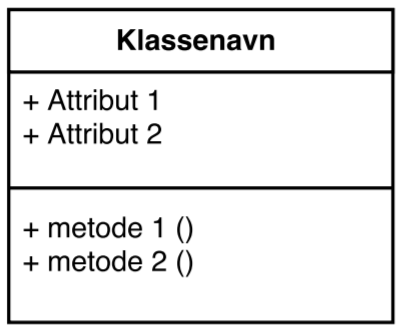
\includegraphics[width=0.5\textwidth]{figures/klassediag}
\caption{}
\label{fig:klassediagram}
\end{figure}